%% 
%% 
%% 

\chapter{Application: Multi-timescale Sequence Learning on Robots
  Simulation Environments}
\chaptermark{Application: SA on Robots Environments}
\label{cha:sa_app}

In this section, we design experiments to answer three questions:
1) Can SA outperform other baselines (regarding episodic returns,
stability, and scalability)? 2) Can SA temporally extend skills
without the termination function? 3) Can skill context vectors be
easily interpreted? 4) Does skill embeddings learned by SA have a
performance boost over other option variants in transfer learning
settings?

For single task learning, experiments are conducted on all OpenAI
Gym MuJoCo environments (10 environments)
\cite{brockman2016openai}. We follow DAC~\cite{zhang2019dac} and
compare our algorithm with five baselines, four of which are
option implementations, i.e., DAC+PPO \cite{zhang2019dac},
AHP+PPO \cite{levy2011unified}, PPOC
\cite{klissarov2017learnings} and OC \cite{bacon2017option}. The
last baseline is PPO \cite{schulman2017proximal}. All baselines'
parameters used in DAC\footnote{All baselines' implementations
  are from DAC's open source repo
  https://github.com/ShangtongZhang/DeepRL/tree/DAC. Note that
  the author list of this paper does not have any overlap with
  DAC. Our source code is available in supplementary materials.}
remain unchanged other than the maximum number of training steps:
SA only needs 1 million steps to converge rather than the 2
million used in DAC. For transfer learning, we follow
\citename{zhang2019dac} and run 6 pairs of transfer learning
tasks constructed in DAC based on DeepMind Control Suite
\cite{tassa2020dmcontrol}. For a fair comparison, we use four
skills for SA and four options for other option implementations.
All experiments are run on an Intel® Core™ i9-9900X CPU @ 3.50GHz
with a single thread and process. Our implementation details are
summarized in \Secref{sec:append_implement}.

\section{Single Task Learning}
\label{sec:exp_perf}
\subsection{Performance}
% towrite: figure capitalize
In Figure \ref{fig:all_tasks}, we report episodic returns on
infinite horizon (i.e., HalfCheetah, Swimmer, HumanoidStandup and
Reacher) and finite horizon (the other tasks) \footnote{We refer
  to environments with the game-over condition as finite horizon
  environments, and infinite vice versa.} environments
separately. For a fair comparison, we use exactly the same
plotting script as used in DAC: curves are averaged over 10
independent runs and smoothed by a sliding window of size 20.
Shaded regions indicate standard deviations.
\begin{figure*}[h]
  \centering
  \includegraphics[width=1\linewidth]{./Part1/figures/all_exps.png}\\
  \caption{\label{fig:all_tasks} Performance of Ten OpenAI Gym
    MuJoCo Environments.}
\end{figure*}
\clearpage
\begin{table*}[]
\caption{Performance of Infinite Horizon Environments}
\label{table:single_infinite}
\vskip 0.15in
\begin{center}
\begin{tabular}{|l|l|l|l|l|}
\hline
        & HalfCheetah        & Swimmer           & HumanoidStandup     & Reacher          \\ \hline
PPO     & 2143.6                & 59.9                 & 62262.2                & -7.5                \\ \hline
DAC+PPO & 1830.1                & 85.0                 & 38954.9                & -8.1                \\ \hline
AHP+PPO & 1701.7                & 86.7                 & 38684.9                & -7.3                \\ \hline
PPOC    & 1441.2                & 43.6                 & 39841.7                & -9.4                \\ \hline
OC      & 832.3                 & 33.0                 & 52352.7                & -15.3               \\ \hline
SA+PPO  & {\ul \textbf{3446.7}} & {\ul \textbf{107.8}} & {\ul \textbf{91654.5}} & {\ul \textbf{-4.6}} \\ \hline
\end{tabular}
\end{center}
\vskip -0.1in
\end{table*}

\begin{table*}[]
\caption{Performance of Finite Horizon Environments}
\label{table:single_finite}
\vskip 0.15in
\begin{center}
\resizebox{1\columnwidth}{!}{%
\begin{tabular}{|l|l|l|l|l|l|l|}
\hline
        & Walker2d           & Hopper             & InvertedPendulum  & InvertedDoublePendulum & Ant                & Humanoid          \\ \hline
PPO     & 1512.5                & 1489.9                & 939.9                & 7112.6                    & 1049.6                & 562.1                \\ \hline
DAC+PPO & {\ul \textbf{1968.0}} & 1702.2                & {\ul \textbf{943.7}} & 5804.5                    & 985.8                 & 487.6                \\ \hline
AHP+PPO & 1520.6                & {\ul \textbf{1993.6}} & 940.0                & {\ul \textbf{7120.7}}     & {\ul \textbf{1359.3}} & {\ul \textbf{569.3}} \\ \hline
PPOC    & 756.1                 & 1308.1                & 936.2                & 7117.6                    & 429.4                 & 483.9                \\ \hline
OC      & 391.9                 & 487.6                 & 207.1                & 2369.4                    & 433.4                 & 475.1                \\ \hline
SA+PPO  & 1856.9                & 1955.3                & 906.5                & 6884.1                    & 907.4                 & 528.7                \\ \hline
\end{tabular}%
}
\end{center}
\vskip -0.1in
\end{table*}

It is extremely interesting that SA shows two completely
different kinds of behaviors on infinite and finite horizon
environments. According to previous option framework
implementations~\cite{klissarov2017learnings,smith2018inference,harb2018waiting,zhang2019dac},
on single task environments, option-based algorithms do not have
a distinguishable performance boost over hierarchy-free
algorithms. SA also has similar behavior and achieves comparable
performance to the best baseline algorithm on most finite horizon
environments (Figure~\ref{fig:all_tasks}). In
\Secref{sec:append_gist} we conceptually explain that
conventional value functions are insufficient to approximate
models which have temporal latent variables dependencies. A
concrete deep wide skill-action architecture remains open for the
future work.

On infinite horizon environments as shown in
Figure~\ref{fig:all_tasks} (a), SA's performance significantly
outperforms all baselines by a large margin in various aspects.
For episodic return, e.g., HumanoidStandup, all option
implementations barely converge, while SA is $240\%$ better than
DAC and AHP\footnote{Even on Reacher, a simple environment on
  which most algorithms converge to a similar performance, SA is
  still $38\%$ better than the second best (AHP).}. For
convergence, SA has the fastest convergence speed. On the first
two environments, which are also reported in DAC, SA only takes
$40\%$ of time steps of DAC and AHP to reach similar episodic
returns. This acceleration is because: 1) SA is MDP formulated,
the skill policy is updated at each time step; 2) SA only has one
action policy decoder; 3) the action decoder learns to decode
skill context vectors whichever skill is activated. For
stability, all 10 runs of SA converge to a similar level while
the other have much larger standard deviations. This property is
theoretically justified by Proposition~\ref{prop:var_red} and
further discussed in \Secref{sec:append_gist}.

\subsection{Temporal Extension}
\label{sec:exp_ext}

It is logical to ask whether SA is capable of temporal extension
without the termination function. To illustrate this, we plot the
average duration of each skill during training episodes of the
HalfCheetah environment in Figure~\ref{fig:duration} (a) and 4
runs of skill activation sequences in
Figure~\ref{fig:option_pattern}. In Figure~\ref{fig:duration}, we
plot the average duration of each skill during 430 training
episodes (each episode contains a trajectory of 512 time steps)
of the HalfCheetah environment. In this environment, the agent
learns to run half of a Cheetah by controlling 6 joints: back
thigh, back shin, back foot, front thigh, front shin, and front
foot. The faster the Cheetah runs forward, the higher return it
gets from the environment.

At the start of training, all skills' durations are short. After
the $100$-th episode, Skill 2's duration quickly grows and
dominates the entire episode. This growth of duration proves that
SA can still temporally extend a skill.

The dominant skill phenomenon is also reported in other option
implementations such as DAC. One explanation for this domination
phenomenon is that for some single task environments, primitive
actions might be enough to express the optimal policy, in which
case extra levels of abstraction (skills) become overhead.
However, towards the end of the training, the dominant skill's
duration starts to decrease while the duration of a secondary
skill (Skill 1) starts to increase. These facts indicate that SA
has a better capability of automatically discovering abstract
actions from primary actions as well as coordinating between
them. The dominant skill phenomenon is also reported in other
option implementations such as DAC. However, as shown in the
video\footnote{https://www.youtube.com/watch?v=QiLVZvI6NJU}, SA
still learns distinguishable skills. Skill 2 is the running
forward skill thus it dominates the whole episode. Skill 1 is
only used to recover from falling down thus it has much shorter
duration. As discussed in \Secref{sec:append_gist},
solution to the dominant skill is actually learning skills at
much finer granularity. The SA-style wide value function
(Eq.~(\ref{eq:sa_v})) provides an elegant solution to this
problem.
\begin{figure*}[h]
  \centering
  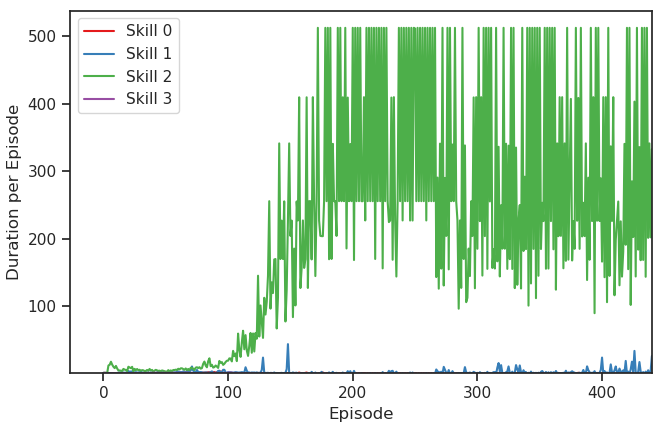
\includegraphics[width=0.7\linewidth]{./Part1/figures/duration.png}\\
  \caption{\label{fig:duration} Duration of 4 options during 430
    training episodes of HalfCheetah.}
\end{figure*}

To illustrate how SA coordinates skills, we take the HalfCheetah
model trained after 1 million steps and independently run it 4
times (4 episodes. each episode contains 512 time steps). Skill
activation sequences of 4 runs are then plotted in
Figure~\ref{fig:option_pattern}.
\begin{figure*}[h]
  \centering
  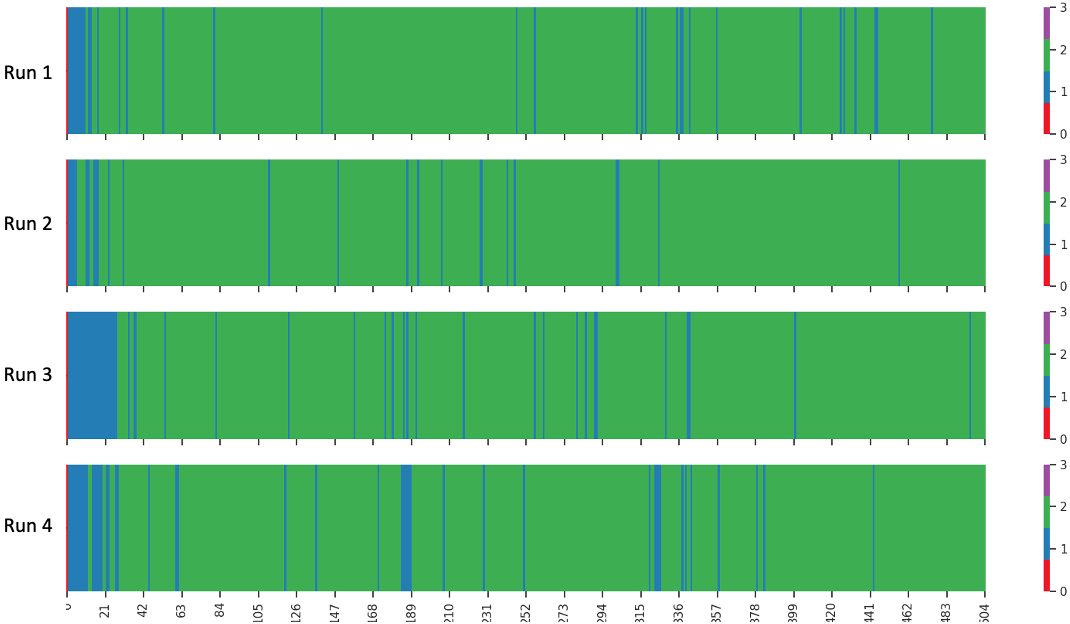
\includegraphics[width=0.7\linewidth]{./Part1/figures/option_pattern.png}\\
  \caption{\label{fig:option_pattern} Activated option sequences
    of 4 independent HalfCheetah runs.}
\end{figure*}
As we can see that there are some common patterns between all 4
independent runs. For example, all runs start with Skill 0 and
use Skill 1 at the early stage. After executing Skill 1 for a
short period, they all switch to Skill 2 which has longest
durations in all 4 runs. From time to time they will fall back to
Skill 1 for short periods and quickly switch to Skill 2 again.
This pattern of coordination indicates that Skill 1 and Skill 2
have completely different functionality and SA has the capability
of automatically discovering as well as leveraging those skills.

\subsection{Interpretation of Skill Context Vectors}
\label{sec:interpret}

In this section we continue with the HalfCheetah model used in
Section~\ref{sec:exp_ext} and demonstrate how to interpret skill
context vectors as well as skill activation sequences (Figure
\ref{fig:option_pattern}). In HalfCheetah, the agent learns to
run half of a Cheetah by controlling 6 joints: back thigh, back
shin, back foot, front thigh, front shin, and front foot. The
faster the Cheetah runs forward, the higher return it gets from
the environment. We interpret skill context vectors and
activation patterns by first inspecting what property each
dimension of the skill context vector encodes (Figure
\ref{fig:first_dim_perturb}). Once each dimension is understood,
skills (Figure \ref{fig:all_skill_vectors}) become straight
forward to interpret by simply inspecting on which dimension
(property) they have the most significant weights (Figure
\ref{fig:interp_skill}). These interpretations can further be
taken to explain skill activation patterns in Figure
\ref{fig:option_pattern}.
\begin{figure*}[h]
  \centering
  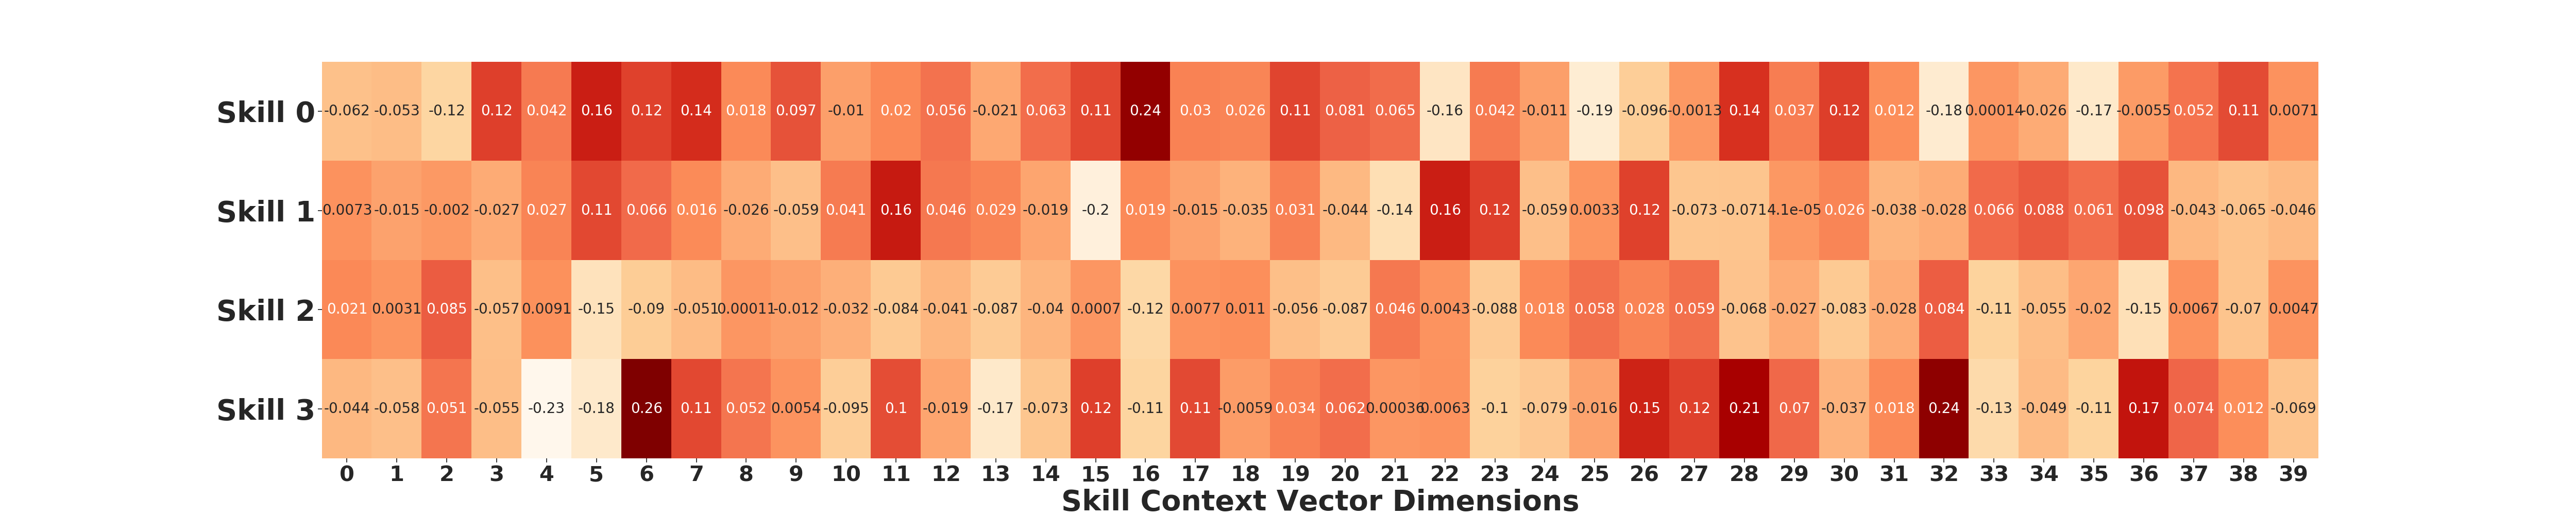
\includegraphics[width=1\linewidth]{./Part1/figures/all_skill_vectors.png}\\
  \caption{\label{fig:all_skill_vectors} Heatmap of all 4 skill
    context vectors}
\end{figure*}

As the first step, we follow \citename{sabour2017dynamic} to
interpret what property each dimension of the skill context
vector in Figure~\ref{fig:all_skill_vectors} encodes by
perturbing each dimension and decode perturbed skill context
vectors into primary actions. Specifically, we perturb one
dimension by adding a range of perturbations $[{-0.1}, 0.09]$ by
intervals of $0.01$ onto it while keep the other dimensions
fixed. After perturbation, each skill context vector dimension
has $20$ perturbed vectors. We then use the action policy decoder
to decode all those vectors into primary actions and see how the
perturbation affects the primary action. As an illustration, we
plot Dimension 0's all $20$ perturbed results in Figure
\ref{fig:first_dim_perturb}.
\begin{figure*}[h]
  \centering
  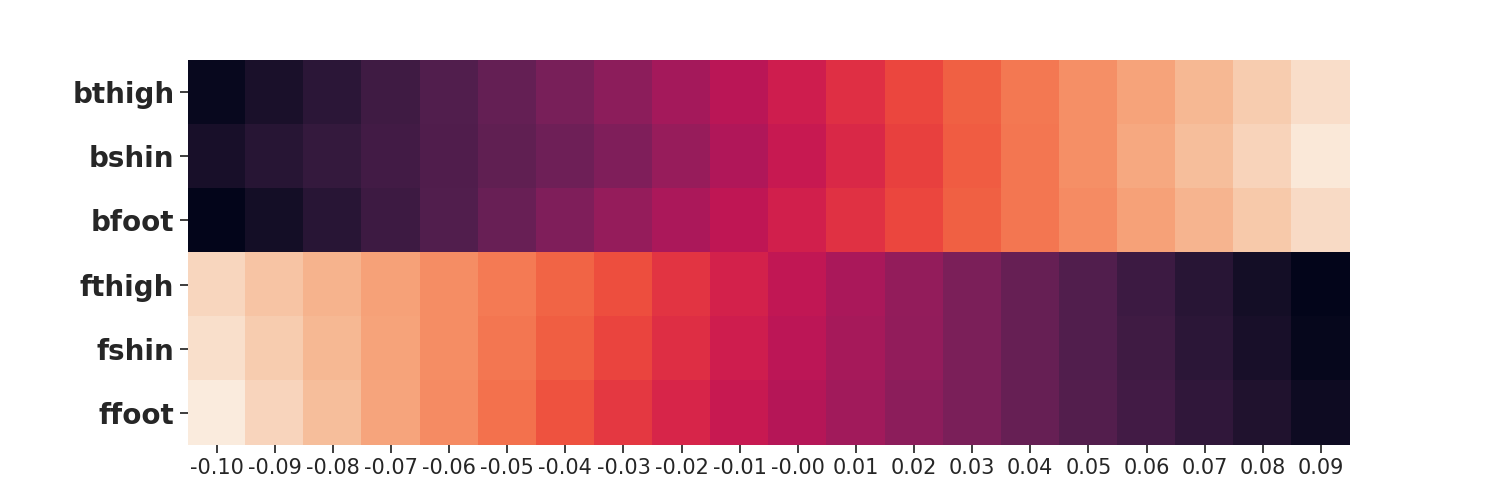
\includegraphics[width=1\linewidth]{./Part1/figures/skill_heatmap.png}\\
  \caption{\label{fig:first_dim_perturb} Perturbation on the
    Dim 0}
\end{figure*}

With visualization of perturbation results in hand, we can
interpret what property each dimension encode by inspecting
relationships between perturbations and primary actions. In
Figure \ref{fig:first_dim_perturb}, as an example, it is clear
that changes on Dim $0$ has opposite effect on the back leg and
front leg: a larger value on Dim $0$ will assign the back leg a
larger torque while the front leg a smaller one, and vice versa.
This means Dim $0$ is has a focus point property: it focuses
torque on only one leg.

Once we know how to interpret one dimension, we can move on to
interpret the whole skill context vector. Since Skill $1$ and
Skill $2$ are two main skills employed in
Figure~\ref{fig:option_pattern}, here we provide an example of
how to interpret them. Figure~\ref{fig:all_skill_vectors} shows
that Skill $1$ has significant values on dimension $11$, $15$ and
$22$. Skill $2$ is significant on dimension $2$, $5$ and $36$. We
demonstrate these dimensions in the same manner as
Figure~\ref{fig:first_dim_perturb} below:
\begin{figure*}[h]
  \centering
  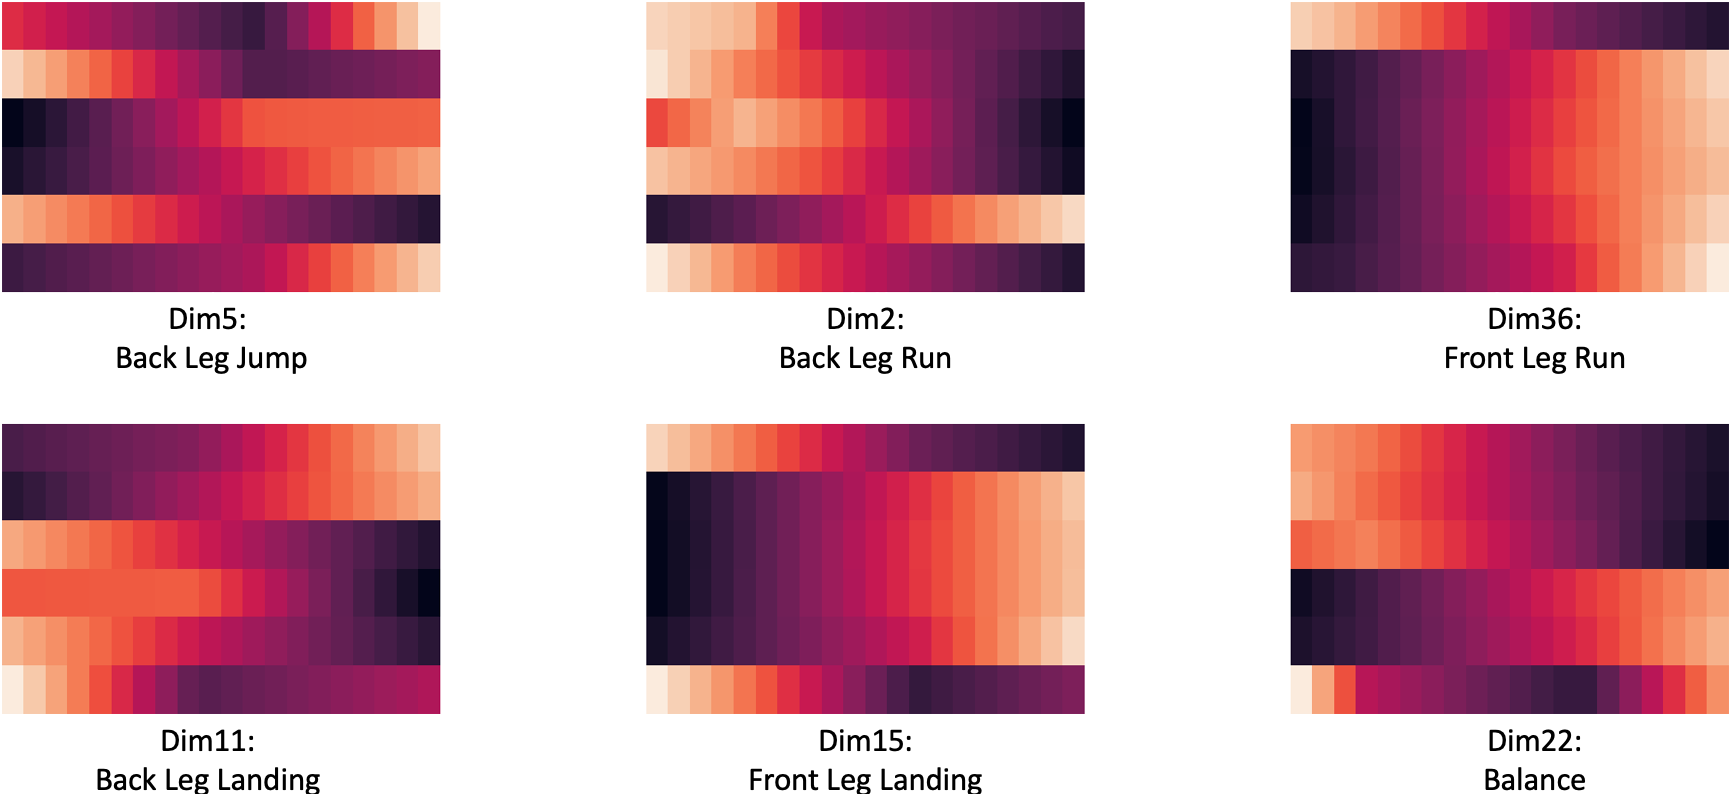
\includegraphics[width=1\linewidth]{./Part1/figures/interp_2_skills.png}\\
  \caption{\label{fig:interp_skill} Interpretation of Skill 1
    and Skill 2}
\end{figure*}

Subfigures in Figure~\ref{fig:interp_skill} can be interpreted in
the same manner as Figure~\ref{fig:first_dim_perturb}. As an
example, from Figure~\ref{fig:all_skill_vectors} we can see that
Skill $1$ has a significant small value on Dim $11$. In
Figure~\ref{fig:interp_skill}, it shows that a smaller Dim $11$
will twist the front leg forward and back foot forward while
twist back thigh, back shin backward. Composition of these
movements is a back leg landing property. Similarly, we can
interpret that Dim $15$ is a front leg landing property and Dim
$22$ is a balancing property. Therefore, Skill $1$ is focusing on
landing from all positions.

Unlike other skill context vectors which have apparent focusing
dimensions, Skill $2$ has a rather balanced skill context vector.
It has no apparently dominant dimension. It only has slightly
more significant values on Dim $2$, $5$, $36$, which are focusing
on jumping and running properties. Therefore, Skill $2$ is more
like an ``all-weather'' skill: it is a skill having very balanced
properties with a slightly demonstration on running and jumping.

Interpretations of Skill $1$ and $2$ above can then be taken to
understand skill activation patterns in
Figure~\ref{fig:option_pattern}: as an all-weather skill, Skill
$2$ is the most frequently executed one and has the longest
duration. From time to time, when the Cheetah needs to land and
balance itself, Skill $1$ will be executed. However, since
landing skill does not provide power of moving forward and thus
has lower returns to continue, once the body is balanced the
Cheetah will quickly stop Skill $1$'s execution and keep running
with Skill $2$.


\section{Transfer Learning}
\label{sec:transfer}

We follow \citename{zhang2019dac} and run 6 pairs of transfer
learning tasks constructed in DAC based on DeepMind Control Suite
\cite{tassa2020dmcontrol}. Each pair contains two different
tasks. To keep consistent with DAC, we train all models one
million steps on the first task and switch to the second (SA's
skill context matrix is subsequently frozen) to run another one
million steps. Results are reported in Figure~\ref{fig:transfer}
(Table~\ref{table:transfer}). On the first task, SA's
performance is among the best algorithms in all environments.
This further validates SA's advantages on single task as observed
in section~\ref{sec:exp_perf}. On the transfer learning (the
second) task, SA's performance ranks the first in 5 out of 6
environments. This shows SA's advantages in knowledge reuse
tasks.
\begin{figure*}[h]
  \vspace{-2mm}
  \centering
  \includegraphics[width=1\linewidth]{./Part1/figures/transfer.png}\\
  \vspace{-4mm}
  \caption{\label{fig:transfer} Performance on DAC transfer
    learning tasks}
  \vspace{-4mm}
\end{figure*}

\begin{table*}[h]
\caption{Performance of Deepmind Control Suite Transfer Learning Environments}
\label{table:transfer}
\begin{center}
\begin{tabular}{|l|l|l|l|l|l|l|}
\hline
        & CartPole             & Reacher              & Cheetah              & Fish                 & Walker1              & Walker2              \\ \hline
PPO     & 829.7                & 327.6                & 73.0                 & 287.9                & 231.8                & 72.2                 \\ \hline
DAC+PPO & 970.8                & 517.2                & 211.2                & 505.4                & {\ul \textbf{590.3}} & 360.5                \\ \hline
AHP+PPO & 966.5                & 395.2                & 167.4                & 357.9                & 362.1                & 143.2                \\ \hline
PPOC    & 942.1                & 400.1                & 72.7                 & 336.7                & 236.6                & 80.9                 \\ \hline
OC      & 106.1                & 19.4                 & 100.6                & 286.6                & 356.3                & 238.7                \\ \hline
SA+PPO  & {\ul \textbf{974.1}} & {\ul \textbf{675.3}} & {\ul \textbf{233.8}} & {\ul \textbf{562.1}} & 473.8                & {\ul \textbf{403.0}} \\ \hline
\end{tabular}
\end{center}
\end{table*}

\section{Conclusions}
\label{sec:conclusion}

In this paper, we presented a novel MDP equivalence of the SMDP
formulated option framework, from which an MDP implementation of
the option framework, i.e., the Skill-Action architecture, was
derived. We theoretically proved that SA has lower variance than
conventional RL models and provided policy gradient theorems for
updating SA. Our empirical studies on challenging infinite
horizon robot simulation environments demonstrated that SA not
only outperforms all baselines by a large margin, but also
exhibits smaller variance, faster convergence, and good
interpretability. On transfer learning, SA also outperforms the
other models in 5 out of 6 environments and shows its advantages
in knowledge reuse tasks.

The final and most important contribution of SA is hierarchically
learning explicit abstract actions' representations with ``skill
context vectors''. This design significantly improves the
scalability and interpretability of SA. It is straightforward to
extend SA to deeper and wider (\Secref{sec:append_gist})
architectures, which gives rise to a large-scale pre-training and
transfer learning architecture in the reinforcement learning
area.

Experiments also show that SA shares two innate limitations with
the conventional option framework
\cite{levy2011unified,klissarov2017learnings,smith2018inference,harb2018waiting,zhang2019dac}:
(1) failure to improve the performance and the sample efficiency
on finite horizon environments (section~\ref{sec:exp_perf}); (2)
``the dominant skill problem'' \cite{zhang2019dac} (section
\ref{sec:exp_ext}). In \Secref{sec:append_gist} we
conceptually discuss that SA-style wide (higher-order
dependencies) value functions could be a solution to both
limitations. This is mainly because these limitations are caused
by the insufficiency of the conventional value functions in
approximating values that have temporal latent variables
dependencies (discussed in \Secref{sec:append_gist}).


\section{Discussion: Learning Skills at Multi-levels of
  Granularity}
\label{sec:append_gist}

Implementations of the option framework share some common
limitations. When proposing the option framework,
\citename{sutton1999between} expected that learning at
multi-level of temporal abstraction should be in favor of faster
convergence and better exploration. On the contrary, significant
improvements on single task environments have not been witnessed
in most option
implementations~\cite{klissarov2017learnings,smith2018inference,harb2018waiting,zhang2019dac}.
To the best of our knowledge, SA is the first option
implementation in which these properties are significantly
witnessed but only on infinite horizon environments. In this
section, we address this problem by first giving a theoretical
explanation of why the value function is the main reason for this
deficiency in section~\ref{sec:append_turkey} and how
\textbf{deep wide value functions} could solve this problem. We
then thoroughly explain the motivations of SA, and why it is a
promising candidate for a deep wide framework, in
section~\ref{sec:append_dwsa}. We also give a further explanation
of how SA is connected to causality reinforcement learning
literature and how a temporal causal reward can be used in
objective to further solve this problem in
section~\ref{sec:append_causal_rew}.

\subsection{Problem Statement and Evidences}
\label{sec:append_turkey}

The expectation of improvements of the option framework on single
task environment builds on an assumption that, by exploiting
hierarchical action and state space, an agent's searching space
can be greatly reduced thus accelerates learning and improving
exploration. However, as reported in section~\ref{sec:exp_ext},
most option frameworks including SA suffer from ``the dominant
skill problem'' \cite{zhang2019dac} which prevents option
frameworks from effectively learning hierarchy in action and
state space as well as coordinating between skills.

One root reason for this problem is that conventional value
functions $V[S_t]$ and $Q[S_t,O_t,A_t]$ make values depend on
temporal latent variables indistinguishable (i.e. Although
different skills $o_1$ and $o_2$ results to different values,
such as $V[S_t,O_{t-1}=o_1]=10$ and $V[S_t,O_{t-1}=o_2]=-10$.
Because they arrive at the same state $S_t$, they have identical
values under conventional value function $V[S_t]=0$). This
deficiency makes option frameworks can only learn skills at very
coarse level thus fail to exploit hierarchical information. The
solution is to use a \textbf{deep wide value function}: enabling
the framework to learn fine-grained skills at mutli-levels of
granularity (deep) and making value functions depend on latent
variables with longer (wide) dependencies (e.g. $V[S_t,O_{t-1}]$
and $Q[S_t,O_t,A_t,O_{t-1}]$).

To have a better understanding the importance of the deep wide
value function, let us consider a simple environment which can be
easily solved by $Q[s_t,a_t,a_{t-1}]$ but not $Q[s_t,a_t]$.

Suppose we are training a robot which only has a camera sensor to
cook thanksgiving turkey. In this setting there are only two
states:
% 
$$\sS=\{\text{Raw Turkey Image},\text{Cooked Turkey
  Image}\}$$
%
The robot's action space only consists of two
actions:
%
$$\sA=\{\text{Stuff turkey},\text{Roast turkey}\}$$
%
As for reward, if the robot roasted a stuffed turkey, then the
reward is $10$. However, if the robot roasted an un-stuffed
turkey, then the reward is $-10$. The $\text{stuff turkey}$
action receives $0$ reward.

The difficulty in this environment is, since the robot only has a
camera to capture an image of the turkey, it can only observes
either $\{\text{Raw Turkey Image}\}$ or $\{\text{Cooked Turkey
  Image}\}$. There is no way to look inside the turkey and see if
the turkey is stuffed. Under this setting, a robot can never
learn to first stuff a turkey and then roast it because
$Q[\text{Raw Turkey Image},\text{Stuff Turkey}] = Q[\text{Raw
  Turkey Image},\text{Roast Turkey}] = 0$. Therefore, the robot
can only randomly cook a turkey. However, this problem can be
easily solved by using a deep wide value function
$Q[S_t,A_t,A_{t-1}]$.

The core problem in this setting is, action has no effect on
states, it only affects rewards. At the first glance this is a
Partially Observed MDP (POMDP) problem since the state of whether
the turkey is stuffed is un-observed. This is true in all
reinforcement learning settings without dependencies on latent
variables. However, it goes much deeper in HRL settings.

In HRL, a common formulation is to estimate a latent variable $O$
to encode hierarchical information and makes the policy depends
on it $P(A_t|S_t,O_t)$. Since $O$ is a latent variable, it is
highly likely that at state $S_t$, different latent variable
$P(A_t|S_t,O_t=o_x)$ and $P(A_t|S_t,O_t=o_y)$ emits the same
action $A_t=A_1$, and thus makes the conventional value function
indistinguishable between $o_x$ and $o_y$.

This phenomenon is especially common around the switching time
step of two skills: around switching point, states are usually
compatible with both old and new skills. Conventional value
functions will be especially confused at those moments. This is
exactly what we observed in \Secref{sec:exp_ext}: overall, skill
2 is executed consistently. However, there are some random
switches to skill 1. And the randomization is increased between
around switching time steps. To explicitly show this, we
visualized ``Run4'' into a video
\footnote{$\text{https://www.youtube.com/watch?v=QiLVZvI6NJU}$}.
The skill selection is very random at the beginning of the
episode as well as around the switching point (the 16th second).
These are exactly the most confusing moments of conventional
value functions. This is not a cherry-pick result but a common
problem. Similar patterns can also be observed here
$\text{https://youtu.be/xrfxbI3duBM?t=4}$ in a HumanoidStandUp
environment.

Due to the insufficiency of conventional value functions,
compatible states have to be different enough to cause
distinguishable values of value functions. Therefore, with
conventional value functions, SA is only able to learn very
coarse skills. For example, as shown in \Secref{sec:interpret}
and the video, the HalfCheetah agent is only able learn two
skills: one is to run forward, one is to stand up when fall.
However it is not able to learn more fine-grained skills such as
jump forward and landing. This problem is not limited to SA, but
is a common problem in HRL. The solution is to use deep wide
value functions.

\subsection{Motivations behind SA's Architecture}
\label{sec:append_dwsa}

SA is carefully designed to make the most out of deep wide value
functions. Compared to other HRL frameworks, SA has following
advantages: 

\begin{enumerate}
\item Stable and unbiased estimation: Thanks to
  proposition~\ref{prop:var_unb} and \ref{prop:var_red}, the
  higher the order of the MDPs, the smaller the variance will be.
  The deep wide value functions stays unbiased estimations of
  conventional value functions no matter how many dependencies
  introduced. The current solution in option framework is a
  biased estimation \cite{harb2018waiting} and adding
  hyper-parameters to the framework.
\item Easy to incorporate wide value functions: Incorporating a
  deep wide value function is straightforward, SA's \textbf{skill
    value upon arrival function} is already a wide function. The
  \textbf{skill value function} and the \textbf{skill-action
    value function} can be easily extended to wide function by
  adding a first-order dependency on $\hat{O}_{t-1}$.
\item Easy to incorporate deep value functions: SA is MDP
  formulated, extending SA to multiple hierarchies is
  straightforward.
\item Scalability to long time dependencies: SA is MDP
  formulated, adding more time dependencies is simply to change
  the 1st-order MDP to higher-order MDPs while both value
  functions and gradient theorems stay unchanged; SA is attention
  based, SA can easily attends to thousand time steps without
  adding any extra complexity to neither skill policy nor action
  policy.
\item Scalability to multiple hierarchies of skills: SA is
  attention based and embedding based. Adding skills is as simple
  as adding skill context matrix. In traditional option
  frameworks \cite{riemer2018learning}, the number of option
  (note that each option is a neural network) grows at $O(N^L)$
  complexity of levels ($N$ is the number of options and $L$ is
  the number of levels).
\item Interpretability. As shown in section~\ref{sec:interpret},
  skill context vectors learned under SA-based architectures are
  straightforward to visualize and interpret. This property is
  especially useful for investigating multi-level granularity
  skills.
\end{enumerate}

\subsection{Causality Discovery Rewards}
\label{sec:append_causal_rew}

Although theoretically a DWSA can learn multi-level granularity
skills, on-policy optimization algorithm is often insufficient
for learning such models especially in sparse reward
environments. However, SA has a natural connection with causal
reinforcement learning thus can exploits causality as a reward in
objective function to further facilitate fine grained skill
discovery. In this section we explain how skill embedding vectors
learned by SA encodes temporal causality relationships and how to
use them to devise causal rewards.

In causal reinforcement learning area, \citename{doshi2016hidden}
proposed Hidden Parameters MDP (Hi-MDP) in which a skill vector
like hidden parameter vector is introduced to learn abstract
properties from environments. PEARL \cite{rakelly2019efficient}
utilizes meta-learning framework to learn a skill representation
that encodes abstract properties of a task and updates the
framework in an off-policy manner to improve sample efficiency in
transfer learning. \citename{killian2017robust} extended Hi-MDP
by including the hidden parameter vector into transition
probability function. \citename{perez2020generalized} further
extended their work by proposing Generalized Hidden Parameter
MDPs (GHP-MDPs), a causality discovery framework by including
hidden parameter vector into both transition function and value
function.

GHP-MDPs is a special case of SA with number of skills $M=1$.
When $M>1$, SA not only encodes causality relationships between
environments and actions but also temporal causality between
skills. Since the latent variable is modeled as a skill vector,
the distance between different trajectories is straightforward to
be calculated and thus can be used as a causal reward to
encourage fine-grained and disentangled skills' discovery. To the
best of our knowledge, SA is the first RL framework concerns
causality in temporal abstraction sequences. We focus this paper
on proposing SA, the causality rewarded SA will be discussed in
future works.

Another interesting understanding of SA is that, rather than an
implementation of the option framework, SA can also be seen as a
novel capsule network~\citename{kosiorek2019stacked} trained by
policy gradient theorems. In Stacked Capsule Auto-Encoders (SCAE)
\cite{kosiorek2019stacked}, a ``capsule'' vector encodes a
different property (scale, orientation, etc.) of the visual
object in each dimension. \citename{kosiorek2019stacked} proposed
to delegate the complexity of part objects detection and
part-to-whole objects aggregation by employing the attention
mechanism \cite{lee2019set} on which a generative model is then
built to further decode the whole-part relationships. This design
choice abstracts the complexity of inference away from the
decoder and largely simplified the designation of the generative
model.

In this paper, we follow their motivations of learning better
representations and utilizing the attention mechanism to simplify
the inference problem (sampling new skill without termination
function). Moreover, the skill context vector is analogously to a
capsule and the skill-action relationship is analogously to the
whole-part relationship in the SCAE. Similar to SCAE utilizing
the equi-variance property of the whole-part relationship to
achieve computing efficiency and better performance, it will be
very exciting to investigate potentially ``equi-variance'' or
``invariance'' properties existed in skill-action relationships,
which might give rise to a novel causal inference architecture in
the reinforcement learning area.
\section{Implementation Details}
\label{sec:append_implement}

In this section we summarize our implementation details. For a
fair comparison, all baselines: DAC+PPO \cite{zhang2019dac},
AHP+PPO \cite{levy2011unified}, PPOC
\cite{klissarov2017learnings}, OC \cite{bacon2017option} and PPO
\cite{schulman2017proximal} are from DAC's open source Github
repo: https://github.com/ShangtongZhang/DeepRL/tree/DAC.
Hyper-parameters used in DAC~\cite{zhang2019dac} for all these
baselines are kept unchanged.

\textbf{SA Architecture:} For all experiments, our implementation
of SA is exactly the same as Figure~\ref{fig:sa_net} (b). We use
Pytorch to build neural networks. Specifically, for skill policy
module, we use a skill context matrix $\mW_S\in \sR^{4\times 40}$
which has $4$ skills ($4$ rows) and an embedding size of $40$
($40$ columns). For Multi-Head Attention, we use Pytorch's
built-in MultiheadAttention
function\footnote{https://pytorch.org/docs/stable/generated/torch.nn.MultiheadAttention.html}
with $num\_heads=1$ and $embed\_dim=40$. For layer normalization
we use Pytorch's built-in function LayerNorm
\footnote{https://pytorch.org/docs/stable/generated/torch.nn.LayerNorm.html}.
For Feed Forward Networks (FNN), we use a 2 layer FNN with ReLu
function as activation function with input size of $40$, hidden
size of $64$, and output size of $64$ neurons. For Linear layer,
we use built-in Linear
function\footnote{https://pytorch.org/docs/stable/generated/torch.nn.Linear.html}
to map FFN's outputs to $4$ dimension. Each dimension acts like a
logit for each skill and is used as density in Categorical
distribution\footnote{https://github.com/pytorch/pytorch/blob/master/torch/distributions/categorical.py}.
For both action policy and critic module, FFNs are of the same
size as the one used in the skill policy.

\textbf{Preprocessing:} States are normalized by a running
estimation of mean and std.


\textbf{Hyperparameters of PPO:} For a fair comparison, we use
exactly the same parameters of PPO as DAC. Specifically:
\begin{itemize}
\item Optimizer: Adam with $\epsilon= 10^{-5}$ and an initial
  learning rate $3 \times 10^{-4}$

\item Discount ratio $\gamma$: $0.99$

\item GAE coefficient: $0.95$

\item Gradient clip by norm: $0.5$

\item Rollout length: $2048$ environment steps

\item Optimization epochs: $10$

\item Optimization batch size: $64$

\item Action probability ratio clip: $0.2$
\end{itemize}


\textbf{Computing Infrastructure:} We conducted our experiments
on an Intel® Core™ i9-9900X CPU @ 3.50GHz with a single thread
and process with PyTorch.


%%% Local Variables:
%%% mode: latex
%%% TeX-master: "../thesis"
%%% End:
